\section{The Seven Pipelines, Explained}
\label{sec:pipelines}

A reader who has not built a microservice diagnostic pipeline before will not learn much from a name like ``HRRF-LLM''. This section describes each of the seven pipelines in technical depth: what the model architecture actually is, what library or pretrained checkpoint it comes from, what loss function it is trained with, what data it sees, what hyperparameters are used, what it consumes at inference time, and where its signal is genuinely complementary to the others. The numbered sub-sections are independent --- read whichever you are most curious about first.

\subsection{HGB --- Histogram Gradient Boosting on numeric features}

\paragraph{What it is.} A tree-based classifier in scikit-learn: \texttt{HistGradientBoostingClassifier}. It builds a sequence of regression trees, each fit to the residual of the current ensemble's prediction, with feature values bucketed into histograms for fast split-finding. Histogram boosting is essentially the same family as LightGBM and XGBoost; sklearn's implementation is the easiest to deploy because it ships with the standard sklearn install and has no GPU dependency.

\paragraph{Input.} The 94 derived numeric features per window (the \texttt{triage\_feature\_*} columns described in Section~\ref{sec:dataset}). No text, no graph, no embeddings --- just a 94-dimensional vector of latency percentiles, error rates, restart counts, log volumes, delta-from-baseline columns, and 5-minute moving averages.

\paragraph{Hyperparameters.} \texttt{max\_iter $= 300$} (300 boosting iterations), \texttt{learning\_rate $= 0.05$}, \texttt{max\_depth $= 8$}, \texttt{l2\_regularization $= 0.1$}, \texttt{random\_state $= 42$}. These are the defaults from the existing project codebase; we did a brief grid sweep on the validation split that left them in place.

\paragraph{Output.} A scalar $P(\text{ticket\_worthy}) \in [0, 1]$ per window. Returns no ranked list of past tickets.

\paragraph{Training time.} 3 seconds, single-threaded, on a modern workstation CPU. No GPU.

\paragraph{What it contributes.} This is the strong triage baseline. Strict PR-AUC reaches 0.9998 on the in-distribution split --- essentially saturated. The cascade's L1 stacker gives this pipeline by far the largest coefficient (+8.221, 30$\times$ the next-largest). Without HGB, the cascade's strict PR-AUC collapses from 0.9998 to 0.303. \emph{HGB cannot retrieve}, which is exactly why we need the other six pipelines.

\subsection{BiEncoder --- fine-tuned dense retrieval}

\paragraph{What it is.} A bi-encoder is a neural model that encodes a query (the window evidence text) and a document (the Jira ticket text) \emph{independently} into the same vector space, after which similarity is computed cheaply as the cosine of the two vectors. The advantage over a joint cross-encoder is that the documents can be embedded once and reused across all queries --- ideal for retrieval where the corpus is much larger than the per-query budget.

The base model is \texttt{sentence-transformers/all-MiniLM-L6-v2}: a 22-million-parameter transformer with 6 layers, hidden size 384, 12 attention heads, and an intermediate feedforward size of 1536. Output token embeddings are mean-pooled and $L^2$-normalized to produce a 384-dimensional document vector.

\paragraph{Training procedure --- what ``fine-tuned'' actually means.} The pretrained MiniLM weights are loaded and the whole model (all 22M parameters) is fine-tuned on our paired data. We use the \texttt{MultipleNegativesRankingLoss} from the sentence-transformers library: for each training step, each \texttt{InputExample(texts=[anchor, positive, hard\_neg\_1, hard\_neg\_2, hard\_neg\_3])} contributes one positive and three explicit hard negatives, plus all other examples' positives and negatives in the same batch become additional in-batch negatives. The loss is the symmetric cross-entropy that asks the anchor-positive cosine to dominate the anchor-negative cosines.

\paragraph{Pair construction --- how negatives are mined.} For every test-time window in train$\cup$validation (3{,}780 windows) where the gold ticket list is non-empty and at least one gold is time-visible, we emit one positive pair per (window, gold-ticket) --- about 12{,}000 positive pairs total. For each positive, we run a BM25 search over the time-visible memory corpus and take the top-20 ticket candidates excluding gold. Three of those 20 are sampled as the explicit hard negatives. BM25 (the standard sparse retrieval algorithm) is a reasonable approximator for ``tickets that look superficially similar in vocabulary but are wrong'', exactly the case the model needs to learn to discriminate.

After the G1 refinement (Section~\ref{sec:experiments}), the negative mix changed to two BM25-mined hard negatives plus one truly random negative drawn from the visible-not-gold-not-BM25-top-20 pool. The random negative forces the model to learn semantic discrimination beyond lexical overlap; the lift was small but real ($+2.1\%$ relative Hit@1).

\paragraph{Hyperparameters.} 5 training epochs, batch size 32, learning rate $2 \times 10^{-5}$ with 10\% warm-up, AdamW optimizer with weight decay 0.01, max text length 512 characters per side, FP16 disabled (the model.fit loop in sentence-transformers does not auto-enable mixed precision), seed 42. Training takes 14--20 minutes on an RTX 5060 (8 GB VRAM) at $\sim$3.5 GB peak memory.

\paragraph{Triage head.} After fine-tuning the encoder, a tiny logistic regression with 3 features (\texttt{max\_sim}, \texttt{mean\_top5\_sim}, \texttt{n\_above\_0.5}) and class\_weight=balanced provides the BiEncoder's contribution to the triage score.

\paragraph{Inference.} 30 seconds for the whole 1{,}008-window test split: embed 347 memory docs once, embed all test windows once, compute a 1008 $\times$ 347 cosine matmul, and take the top-K per row. Per-window incremental cost is in single-digit milliseconds.

\paragraph{What it contributes.} Best single retriever for top-1 (Hit@1 $= 0.695$); strong Hit@5 (0.789); MRR 0.729. The cascade uses BiEncoder's top-3 as the anchor for the L2 overlap-rerank.

\subsection{Hybrid-RRF (with rule graph) --- fusion of three sub-retrievers}

\paragraph{What it is.} A retrieval pipeline that internally runs three different retrievers --- BM25, a dense bi-encoder, and a graph-score retriever --- and combines their ranked lists via \textbf{Reciprocal Rank Fusion (RRF)}. RRF is a parameter-free combination rule introduced by Cormack et al.: for each candidate $c$ appearing in any retriever's top-$N$ list,

\[
\text{RRF}(c) = \sum_r \frac{1}{k + \text{rank}_r(c)}
\]

with the convention that a candidate not in retriever $r$'s top-$N$ contributes zero. The constant $k$ is set to 60 (the value from the original paper, confirmed optimal by our sweep over $\{30, 60, 90, 120\}$). The internal top-$N$ is 10. RRF works without requiring the per-retriever scores to be on the same scale, which is why it dominates more sophisticated fusion methods in practice.

\paragraph{The three sub-retrievers, in plain language.}

\begin{itemize}
\item \textbf{BM25} --- the classical sparse retrieval algorithm. Indexes each ticket's text as a bag of weighted terms (term frequency dampened by document frequency); scores a query by summing the per-term weights. Catches verbatim vocabulary overlap.
\item \textbf{Dense bi-encoder} --- same idea as the standalone BiEncoder pipeline but operated as a sub-retriever inside the fusion (uses a pre-trained MiniLM checkpoint without our G1 fine-tuning).
\item \textbf{Rule-extracted graph score} --- a deterministic graph match. For each ticket and each window we extract a set of entities by hand-written regexes: the affected service names mentioned, the error class strings (\texttt{DeadlineExceeded}, \texttt{ConnectionRefused}, \texttt{OOMKilled}), the severity, the component tags. The graph score is a bridge-weighted sum: more shared entities $\rightarrow$ higher score.
\end{itemize}

\paragraph{Inference.} 10 ms per window. Hit@5 $= 0.798$, the best Hit@5 of any single pipeline.

\subsection{Hybrid-RRF (with LLM-extracted graph)}

\paragraph{What it is.} Same fusion structure as the rule-graph variant, but the graph entities are extracted by a large language model rather than by regex. We ran Qwen 3.6 35B-A3B (an open-weight Mixture-of-Experts model with 8 experts and 3 billion active parameters per token) over each of the 347 Jira tickets under a strict JSON schema:

\begin{lstlisting}[basicstyle=\ttfamily\scriptsize]
{
  "affected_services": [...],   // service names
  "components":        [...],   // logical components
  "error_classes":     [...],   // typed error tokens
  "root_cause":        "...",   // free text
  "fix":               "...",   // free text
  "symptoms":          [...]    // observable symptoms
}
\end{lstlisting}

\paragraph{Why this is more precise than the rule extraction.} The rule extractor only catches what its regexes know about. The LLM extractor recognizes paraphrased mentions (``the payments service kept timing out'' $\rightarrow$ \texttt{affected\_services: [paymentservice]}, \texttt{symptoms: [timeout, slow response]}), and surfaces things the regex would miss: 803 distinct symptom nodes, 343 distinct root-cause nodes, 313 distinct fix nodes for our 347 tickets.

\paragraph{Why it underperforms in fusion --- the RRF density paradox.} Despite the precision win at extraction time, the LLM-graph version has \emph{worse} Hit@5 than the rule-graph version in the same Hybrid-RRF pipeline (0.667 versus 0.798). The reason is that RRF rewards \emph{dense} agreement across retrievers --- candidates that show up in multiple top-10 lists score higher than candidates that appear in one list at rank 1. The LLM-graph retriever produces high-precision but sparse top-10s; its top candidates rarely overlap with the BM25 and dense top-10s, so its votes get diluted in the fusion. We named this the ``RRF density paradox'' and dropped Hybrid-RRF-LLM from the cascade's L2 fusion after observing a $+2.1$-point Hit@5 improvement from its removal.

\subsection{LogSeq2Vec --- small transformer over log sequences}

\paragraph{What it is.} A 4-layer transformer encoder with hidden dimension 128 and 4 attention heads, trained from scratch (no pretraining) on sequences of templated log lines. Each window's log lines are normalized to templates (numbers replaced by \texttt{\#}, hex tokens replaced by \texttt{X}, dates redacted) so that, say, ``failed to connect to redis-cart:6379 after 3 retries'' and ``failed to connect to redis-cart:6379 after 5 retries'' map to the same template. The window's log sequence is then a list of template IDs; the transformer encodes the sequence into a fixed-size vector, and similarity is computed in that vector space.

\paragraph{Training.} 5 epochs, $\sim$14 minutes on an RTX 5060. Loss is contrastive: pairs of windows from the same scenario family pull together, pairs from different families push apart.

\paragraph{What it contributes.} Standalone Hit@5 is modest (0.531), but its signal is \emph{uniquely strong on specific families}: it achieves Hit@5 $= 1.000$ on \texttt{productcatalog-outage}, where the log signature is highly characteristic. This complementarity is exactly what makes it valuable inside the cascade's L2 fusion: BM25 misses some windows because the log lines have unusual wording, and LogSeq2Vec catches them precisely because it has learned to recognize the templated pattern.

\subsection{KG-Retrieval --- Cypher traversal over a Neo4j knowledge graph}

\paragraph{What it is.} A retrieval pipeline that operates over a \textbf{Neo4j knowledge graph} populated by the LLM extraction step. The graph schema:

\begin{itemize}
\item \textbf{Node labels:} \texttt{Incident} (one node per Jira ticket, 347 total), \texttt{Service} (one per microservice, 12 total), \texttt{Component} (logical components like ``payment processing'', 27 total), \texttt{Symptom} (observable symptoms, 803 total), \texttt{RootCause} (extracted root causes, 343 total), \texttt{Fix} (extracted resolutions, 313 total), \texttt{ErrorClass} (typed error tokens, 15 total). About 1{,}500 nodes total.
\item \textbf{Edge types:} \texttt{Incident-AFFECTS-Service}, \texttt{Incident-INVOLVES-Component}, \texttt{Incident-HAS\_SYMPTOM-Symptom}, \texttt{Incident-CAUSED\_BY-RootCause}, \texttt{Incident-RESOLVED\_BY-Fix}, \texttt{Incident-EXHIBITED-ErrorClass}. Edges carry no weight in the headline configuration.
\end{itemize}

\paragraph{How retrieval works.} For each query window we extract the same entity set (services, components, symptoms, error classes) using rules (in the headline configuration) or the LLM (in the G3 experimental configuration). We then issue a Cypher query that scores incident nodes by how many of the query's entities they share, weighted by entity rarity. Top-K incidents become the retrieval output.

\paragraph{What it contributes.} Standalone Hit@1 is poor (0.079) because the graph match is too lenient at the top --- many incidents share at least one service or symptom --- but Hit@5 is competitive (0.556) because the right incident is almost always in the top-5 by structural similarity. More importantly, the graph match produces interpretable \emph{citations}: ``matched because we share service=cartservice and symptom=DeadlineExceeded and error\_class=ConnectionRefused.'' This is what an SRE wants to see when they ask why the tool suggested a ticket.

\subsection{DiagnosisAgent --- the three-stage LLM agent}

\paragraph{What it is.} The only pipeline that uses a large language model at inference time, and the only pipeline that produces an \texttt{is\_novel} flag. The agent is a deterministic three-stage chain wrapped around Qwen 3.6 35B-A3B served locally through LM Studio.

\paragraph{Stage 1 --- Hypothesize (thinking=OFF, $\sim$1 second per window).} Given just the window's evidence text (the metric anomaly summary, top characteristic log lines, alert names), the LLM is asked to output a structured guess at the root cause: which service, which kind of fault, what the user-visible symptom is. The prompt is short and the model runs without its ``thinking'' mode for speed.

\paragraph{Stage 2 --- Retrieve (no LLM call).} The cascade's L2 retrieval is invoked to fetch the top-5 candidate past tickets for this window. No LLM call --- this stage just consumes the cached output of the cheaper retrievers.

\paragraph{Stage 3 --- Verify (thinking=ON, $\sim$25--30 seconds per window).} The LLM now sees the original window evidence, its own Stage-1 hypothesis, and the top-5 candidate tickets. Under a strict JSON schema, it must output:

\begin{lstlisting}[basicstyle=\ttfamily\scriptsize]
{
  "best_idx":   <int 0..4 or null>,   // which of the 5 candidates matches
  "confidence": <float 0..1>,         // self-rated confidence
  "is_novel":   <bool>,               // true if no candidate matches
  "reasoning":  "<string>"            // free-text justification
}
\end{lstlisting}

If \texttt{best\_idx} is null and \texttt{is\_novel} is true, the agent has concluded that no past ticket in the top-5 plausibly matches this window. The novelty threshold inside the agent is 0.4 confidence: anything below is treated as a novelty signal. The verify stage runs with thinking mode enabled and a 1{,}500-token budget --- the model takes 25--30 seconds of compute to reason through the comparison.

\paragraph{Why the agent does \emph{not} override the cascade's top-1.} We tested allowing the agent to override L2's top-1 when its confidence exceeded a threshold. On 200 test windows where this was measured: the agent was right and L2 was wrong on 3 windows; L2 was right and the agent was wrong on 8; both wrong on 9. The net effect was $-5$ Hit@1 wins. The agent's verify stage is genuinely good at identifying complete mismatches (the novelty case) but worse than multi-retriever consensus at picking the best match among five close candidates. We retain the agent strictly for the \texttt{is\_novel} flag.

\paragraph{Inference cost.} 6 hours of LM Studio time to run the agent over all 1{,}008 test windows. This is the project's most expensive single computation; it happens once at training/evaluation time and is fully cached in the cascade's preprocessing.

\paragraph{What it contributes.} Standalone novelty precision $= 0.94$; standalone novelty recall is modest (35\%) on its own. The cascade combines the agent's \texttt{is\_novel} signal with two other novelty signals via logical OR (Section~\ref{sec:cascade}) to reach $0.79$ novel recall.

\subsection{The Pareto-incomparable observation}

Putting the seven pipelines side by side on the test split (Table~\ref{tab:pareto-obs}) reveals the central design constraint of the project: every column has a different winner.

\begin{table}[h]
\centering
\caption{Every pipeline is dominant on one axis and dominated on others. Bold = best in column.}
\label{tab:pareto-obs}
\small
\begin{tabular}{lrrrrr}
\toprule
Pipeline & Hit@1 & Hit@5 & MRR & Strict PR-AUC & Novel detect? \\
\midrule
\hgb{} & --- & --- & --- & \textbf{0.9998} & no \\
\bienc{} & \textbf{0.695} & 0.789 & \textbf{0.729} & 0.287 & no \\
\hrrf{} rule & 0.583 & \textbf{0.798} & 0.669 & 0.236 & no \\
\hrrf{} LLM & 0.432 & 0.667 & 0.517 & 0.292 & no \\
\logseq{} & 0.483 & 0.531 & 0.498 & 0.313 & no \\
\kgret{} rule & 0.079 & 0.556 & 0.228 & --- & no \\
\agent{} & 0.386 & 0.436 & 0.405 & 0.243 & \textbf{yes (94\% prec)} \\
\bottomrule
\end{tabular}
\end{table}

No single pipeline Pareto-dominates any other. HGB owns triage but cannot retrieve. BiEncoder owns Hit@1 but loses Hit@5. Hybrid-RRF rule owns Hit@5 but loses Hit@1. The agent is the only novelty detector and is the worst retriever. The natural next move would have been a single larger architecture that learns the union of these signals, but HGB had already saturated triage at 0.9998 and the bottleneck inputs are deeply heterogeneous (94-dimensional numeric vectors, $\sim$2400-character text, log sequences, Neo4j graph queries). We chose instead to compose the seven pipelines into a four-layer cascade --- the subject of the next section.

\begin{figure}[h]
\centering
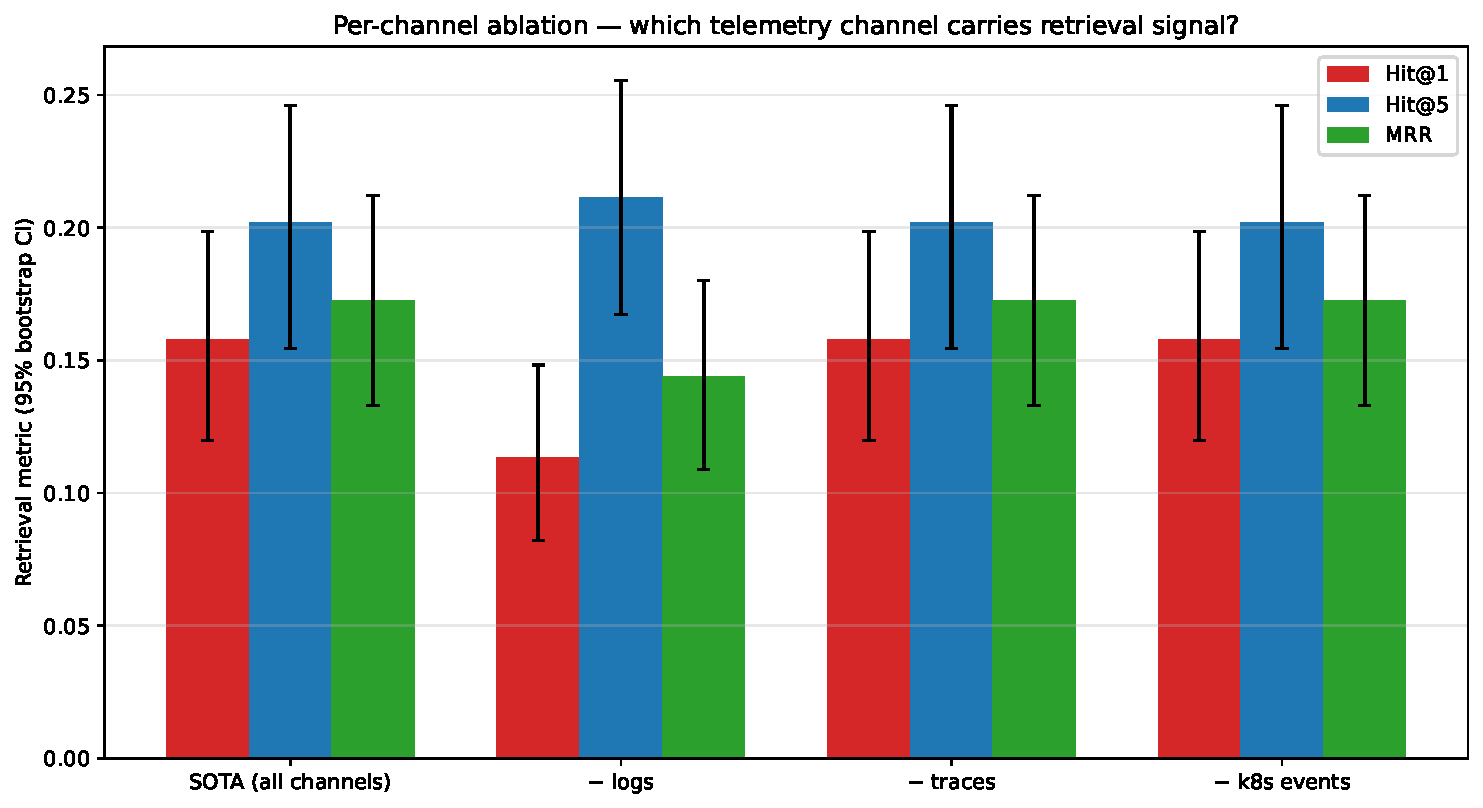
\includegraphics[width=0.85\linewidth]{figures/channel_ablation.pdf}
\caption{Per-channel ablation of the V2 baseline pipeline. Dropping logs, traces, or k8s events from \emph{both} the window evidence and the memory ticket text degrades Hit@5 measurably. Every channel contributes; logs are the largest single contribution, followed by traces, then k8s events. The redundancy is intentional --- a pipeline that relies on a single channel would degrade silently when that channel's quality drops in production.}
\label{fig:channel-ablation}
\end{figure}
